\documentclass[12pt,a4paper]{article}
\usepackage[utf8]{inputenc}
\usepackage{amsfonts}
\usepackage{amssymb}
\usepackage{amsmath}
\usepackage{graphicx}
\usepackage{float}

% sets margin
\usepackage[hmargin=3cm,vmargin=2.5cm]{geometry}

% creates landscape pages
\usepackage{pdflscape}
\usepackage{pdfpages}

%\renewcommand{\rmdefault}{phv} % Arial
\renewcommand{\sfdefault}{phv} % Arial

% defining settings for textpos
\usepackage[absolute]{textpos}
\setlength{\TPHorizModule}{\paperwidth}
\setlength{\TPVertModule}{\paperheight}

% headers / footers
\usepackage{fancyhdr}
\pagestyle{fancy}
\fancyhf{}
\rhead{Assignment 2}
\lhead{CSP2348: Data Structures}
\rfoot{\thepage}
\lfoot{Martin Ponce, ID: 10371381}
\renewcommand{\footrulewidth}{0.5pt}

% defining landscape headers / footers
\fancypagestyle{fancylscape}{
	\fancyhf{}
	\renewcommand{\footrulewidth}{0pt}
	\renewcommand{\headrulewidth}{0pt}
	% header
	\begin{textblock}{0.05}[-0.5,-2](0,0)
		{\rotatebox{90}{CSP2348: Data Structures}}
	\end{textblock}
		\begin{textblock}{0.05}[-0.5,-1](0,0)
		{\rotatebox{90}{Assignment 2}}
	\end{textblock}
	\begin{textblock}{0.05}[-1,-0.109](0,0)
		{\rotatebox{90}{\rule{24.2cm}{0.5pt}}}
	\end{textblock}
	% footer
	\begin{textblock}{0.05}[-19,-4.28](0,0)
		{\rotatebox{90}{Martin Ponce, ID: 10371381}}
	\end{textblock}
		\begin{textblock}{0.05}[-19,-12.8](0,0)
		{\rotatebox{90}{\thepage}}
	\end{textblock}
		\begin{textblock}{0.05}[-18.7,-0.109](0,0)
		{\rotatebox{90}{\rule{24.2cm}{0.5pt}}}
	\end{textblock}
}

% adjusts padding between caption and figure
\setlength{\belowcaptionskip}{10pt}

% adds links to references and colors them blue
\usepackage{hyperref}
\hypersetup{colorlinks=true,
			linkcolor=blue,
			citecolor=black,
			urlcolor=blue}

% apa style referencing
\usepackage[sectionbib, natbibapa]{apacite}
\usepackage{chbibref}

% underlining text
\usepackage[normalem]{ulem}

% \citetapos for possesive citations
\newcommand{\citetapos}[1]{\citeauthor{#1}{\textcolor{black}{'s}} \citeyearpar{#1}}

% add multiline comments \begin{comment} \end{comment}
\usepackage{verbatim}

% add minted package for code highlighting, number per section
\usepackage[section]{minted}

% add tcolorbox package to style code
\usepackage{tcolorbox}
\tcbuselibrary{minted,skins}

% javacode style config
\newtcblisting{javacode}{
  listing engine=minted,
  colback=bg,
  colframe=black!80,
  listing only,
  minted style=monokai,
  minted language=java,
  minted options={linenos=true,texcl=true,fontsize=\scriptsize},
  left=1mm,
}

% consolecode style config
\newtcblisting{consolecode}{
  listing engine=minted,
  colback=bg,
  colframe=black!80,
  listing only,
  minted style=vim,
  minted language=console,
  minted options={texcl=true,fontsize=\scriptsize},
  left=1mm,
}

% define bg color for code highlighting
\definecolor{bg}{rgb}{0.20,0.20,0.20}

% listings package
\usepackage{listings}
% change label to code
\renewcommand\listingscaption{Java code}

% modify enumerate sub list
\renewcommand{\labelenumii}{\theenumii}
\renewcommand{\theenumii}{\theenumi.\arabic{enumii}.}
\renewcommand{\theenumiii}{\theenumii\arabic{enumiii}}
\renewcommand{\theenumiv}{\theenumiii.\arabic{enumiv}}

% number each equation per section
\numberwithin{equation}{section}

% tikz graphics package
\usepackage{tikz}
\usetikzlibrary{arrows,positioning, calc}
\tikzstyle{vertex}=[draw,fill=black!15,circle,minimum size=18pt,inner sep=0pt]

% front matter
\title{Edith Cowan University\\CSP2348\\Data Structures\\Assignment 2}
\author{Martin Ponce\\Student 10371381\\\\Tutor: Jitian Xiao}
\date{\today}

\begin{document}

% title page
\newpage
\null  % Empty line
\nointerlineskip  % No skip for prev line
\vfill
\let\snewpage \newpage
\let\newpage \relax
\maketitle
\thispagestyle{empty}
\let \newpage \snewpage
\vfill

% toc
\newpage
\tableofcontents
\thispagestyle{fancy}

\newpage
\section{Introduction}

The Board of Directors at Blue Ink have recently become aware of the lack of computer security awareness and best practices amongst its employees. As a result, Blue Ink have requested that a sample Virtual Machine (VM) image of a typical computer within their organisation be analysed for security issues.

This report outlines the security issues identified during the analysis of Blue Ink's sample VM image. Vulnerabilities have been found with the operating system itself, and support software packaged with the operating system, such as the Internet browser and anti-virus application. Vulnerabilities have also been identified in outdated software whilst practices regarding the storage of passwords in plain-text files within user documents folders provide opportunities for unwanted access. The security issues identified in this report must be addressed in order to maintain the utmost security.

\subsection{Assumptions}

\begin{itemize}
\item A firewall is implemented within the network
\end{itemize}

\newpage
\section{Arrays}

The array data structure is demonstrated through the implementation of a simple lotto game. The lotto game allows up to 1000 players, with each player picking six unique integers, between 1 and 45, which makes up their lotto ticket. Each player and their respective lotto tickets are represented inside a two-dimensional array, while the winning numbers are represented inside a one-dimensional array.
\\
\\
The following classes have been created to represent the lotto game:

\begin{itemize}
\item \mintinline{java}{Main}: The executable class, contains \mintinline{java}{main()} method
\item \mintinline{java}{PlayerTickets}: Generates a two-dimensional array which represents each player, and their picks for the lotto ticket
\item \mintinline{java}{WinningNumbers}: Generates a one-dimensional array which represents the winning numbers for the lotto game
\item \mintinline{java}{WinningPlayers}: Contains logic to determine who the winning players are, which of their numbers match the winning numbers, and their winner class category
\item \mintinline{java}{Sorter}: Helper class to sort \mintinline{java}{PlayerTickets} and \mintinline{java}{WinningNumbers} arrays
\item \mintinline{java}{Randomizer}: Helper class to generate random numbers for each player pick and winning number
\end{itemize}

\subsection{Sorting}

In order to use more efficient search algorithms such as binary search, the arrays must be sorted first. The merge sort algorithm has been selected due to its time efficiency of $O(n \ log \ n)$. This algorithm is implemented as a static method of the \mintinline{Java}{Sorter} class, as shown in Java code 2.1 and 2.2.

\subsubsection{Merge sort algorithm}

To sort $a$[left...right] into ascending order:

\begin{enumerate}
\item If left $\leq$ right:
	\begin{enumerate}
	\item Let $m$ be an integer about midway between left and right
	\item Sort $a$[left...$m$] into ascending order
	\item Sort $a$[$m+1$...right] into ascending order
	\item Merge $a$[left...$m$] and $a$[$m+1$...right] into auxiliary array $b$
	\item Copy all components of $b$ into a[left...right]
	\end{enumerate}
\item Terminate
\end{enumerate}

\noindent
\citep[p. 54]{Watt2001}


\subsubsection{Merge sort Java method}

\begin{listing}[H]
\caption{Merge sort method}
\begin{javacode}
private static void mergeSort(int low, int high) {

    // 1.0 If left (low) < right (high)
    if(low < high) {

        // 1.1 Let m (mid) be an integer about midway between left and right
        int mid = low + (high - low) / 2;

        // 1.2 Sort a[left...m] into ascending order
        mergeSort(low, mid);

        // 1.3 Sort a[m+1...right] into ascending order
        mergeSort(mid + 1, high);

        // 1.4 Merge a[left...m] and a[m+1...right] into auxiliary array b
        // call merge() which is O(n)
        merge(low, mid, high);
    }
}
\end{javacode}
\end{listing}

\noindent
At line 17, the \mintinline{java}{mergeSort()} method calls supporting method \mintinline{java}{merge()}, as shown in Java code 2.2, in order to perform step 1.4 of the merge sort algorithm.

\begin{listing}[H]
\caption{Merge method}
\begin{javacode}
private static void merge(int low, int mid, int high) {

    // iterate from low through to high
    for(int i = low; i <= high; i++) {

        // copy each element from the array to sort, to each element into temp array
        mergeTempArray[i] = mergeArrayToSort[i];
    }

    // 1.0 Set i = low, set j = mid + 1, set k = low
    int i = low;
    int j = mid + 1;
    int k = low;

    // 2.0 While i <= mid AND j <= high, repeat:
    while(i <= mid && j <= high) {

        // 2.1 If mergeTempArray[i] <= mergeTempArray[j],
        if(mergeTempArray[i] <= mergeTempArray[j]) {

            // 2.1.1 Copy mergeTempArray[i] into mergeArrayToSort[k], then increment i and k
            mergeArrayToSort[k] = mergeTempArray[i];
            i++;

        // 2.2 If mergeTempArray[i] > mergeTempArray[j],
        } else {

            // 2.2.1 Copy mergeTempArray[j] into mergeArrayToSort[k], then increment j and k
            mergeArrayToSort[k] = mergeTempArray[j];
            j++;
        }
        k++;
    }

    // 3.0 While i <= mid,
    while(i <= mid) {

        // 3.1 Copy mergeTempArray[i] into mergeArrayToSort[k], then increment i and k
        mergeArrayToSort[k] = mergeTempArray[i];
        k++;
        i++;
    }
}
\end{javacode}
\end{listing}

\subsubsection{Merge sort analysis}

As \citet[p. 54 - 55]{Watt2001} explain, analysis of the merge sort algorithm's time complexity involves counting the number of comparisons made during the operation. Let $n =$ right $-$ left $+ 1$ be the length of the array, and let $C(n)$ be the total number of comparisons required to sort $n$ values.

Step 1.1 involves dividing the array into two subarrays, $n/2$. The left subarray takes around $C(n/2)$ comparisons to sort, and similarly, the right subarray takes around $C(n/2)$ comparisons to sort.

Step 1.4 involves the merging of each subarray into a sorted array and takes about $n - 1$ comparisons to complete. Therefore:

\begin{equation}
C(n) \approx \left\{\begin{matrix}
2C(n/2) + n - 1 & \mbox{if} \ n > 1 \\ 
0 & \mbox{if} \ n \leq 1 
\end{matrix}\right.
\end{equation}

\newpage
\noindent
Simplifying equation 2.1:

\begin{equation}
C(n) \approx n \times \log_2n
\end{equation}

\noindent
Therefore the time complexity is $O(n \log n)$.
\\
\\
Space complexity is $O(n)$, since step 1.4 requires an auxiliary array of length $n$ to temporarily store the sorted array.

\subsubsection{Merge sort console output}

The following console outputs demonstrate that the merge sort algorithm is functioning correctly, and sorts player lotto picks and winning numbers in ascending order as desired. Note that the examples shown truncate actual results down to ten results from a thousand.
\\
\begin{consolecode}
***********************
*** UNSORTED ARRAYS ***
***********************

Player 0001 picks: [16][14][37][31][07][42]
Player 0002 picks: [20][12][26][23][44][16]
Player 0003 picks: [10][32][20][35][02][24]
Player 0004 picks: [06][23][19][35][42][25]
Player 0005 picks: [07][17][28][41][29][38]
Player 0006 picks: [16][05][36][31][04][23]
Player 0007 picks: [20][01][34][37][07][18]
Player 0008 picks: [30][29][10][27][34][05]
Player 0009 picks: [03][27][13][38][28][32]
Player 0010 picks: [08][24][45][14][02][07]

Winning Numbers:   [21][22][10][03][04][13]
\end{consolecode}

\begin{consolecode}
***********************
**** SORTED ARRAYS ****
***********************

Player 0001 picks: [07][14][16][31][37][42]
Player 0002 picks: [12][16][20][23][26][44]
Player 0003 picks: [02][10][20][24][32][35]
Player 0004 picks: [06][19][23][25][35][42]
Player 0005 picks: [07][17][28][29][38][41]
Player 0006 picks: [04][05][16][23][31][36]
Player 0007 picks: [01][07][18][20][34][37]
Player 0008 picks: [05][10][27][29][30][34]
Player 0009 picks: [03][13][27][28][32][38]
Player 0010 picks: [02][07][08][14][24][45]

Winning Numbers:   [03][04][10][13][21][22]
\end{consolecode}

\newpage
\subsection{Searching}

In order to determine the winners of the lotto game, the program must be able to search each number from the winning numbers array within each array of player tickets. Total number of winners within each winner class category must be calculated and displayed, as well as the result for an individual player, which simulates a player requesting their ticket to be checked for winning numbers.

For both functions to be implemented, two search algorithms have been selected, binary search and an adaptation of the merge array algorithm to sequentially compare components of two sorted arrays. Both of these algorithms may be implemented since the arrays have been sorted in ascending order. These algorithms are implemented as instance methods within the \mintinline{java}{WinningPlayers} class, as shown in Java code 2.3 and 2.4.

\subsubsection{Binary search algorithm}

To find which (if any) component of the sorted (sub)array $a$[left...right] equals target:

\begin{enumerate}
\item Set $l$ = left, $r$ = right
\item While $l \ \leq \ r$, repeat:
	\begin{enumerate}
	\item Let $m$ be an integer about halfway between $l$ and $r$
	\item If target equals $a[m]$, terminate with answer $m$
	\item If target is less than $a[m]$, set $r = m - 1$
	\item If target is greater than $a[m]$, set $l = m + 1$
	\end{enumerate}
\item Terminate with answer none
\end{enumerate}

\noindent
\citep[p. 43]{Watt2001}

\subsubsection{Binary search Java method}

\begin{listing}[H]
\caption{Binary search method}
\begin{javacode}
private int binarySearch(int[] array, int target) {

    // 1.0 Set l = left, and r = right (substituted with low and high respectively)
    int low = 0;
    int high = array.length - 1;

    // 2.0 While l <= r, repeat:
    while(low <= high) {

        // 2.1 Let m (mid) be an integer about midway between l and r
        int mid = low + (high - low) / 2;

        // 2.2 If target equals a[m], terminate with answer m
        if(target == array[mid]) {
            return mid;

        // 2.3 If target is less than a[m], set r = m - 1
        } else if(target < array[mid]) {
            high = mid - 1;

        // 2.4 If target is greater than a[m], set l = m + 1
        } else {
            low = mid + 1;
        }
    }

    // 3.0 Terminate with answer none
    return -1;
}
\end{javacode}
\end{listing}

\subsubsection{Binary search analysis}

Analysis of the binary search algorithm's time complexity involves counting the number of comparisons made during the operation. Let $n =$ right $-$ left $+ 1$ be the length of the array, and assume that steps 2.2 to 2.4 are implemented as a single comparison. At most, these steps are iterated as many times as $n$ can be halved until it reaches 0. Therefore the number of comparisons is $\mbox{floor}(\log_2n) + 1$ \citep{Watt2001}. The time complexity for binary search is $O(\log n)$.

\newpage
\subsubsection{Binary search console output}

The console output below displays the total number of winners in each winner class. To be considered a winner in this lotto game, a player must match at least 3 picks in their ticket to the winning numbers.

Each winner class is categorised by the number of matches a player may have between the picks in their ticket, and the winning numbers:

\begin{itemize}
\item 1st class: 6 picks match winning numbers
\item 2nd class: 5 picks match winning numbers
\item 3rd class: 4 picks match winning numbers
\item 4th class: 3 picks match winning numbers
\end{itemize}

\begin{consolecode}
***********************
**** BINARY METHOD ****
***********************

1st class winners: 0
2nd class winners: 0
3rd class winners: 4
4th class winners: 26
\end{consolecode}

\noindent
The console output below displays results for individual players.
\\
\begin{consolecode}
** BINARY TICKET CHECKING **

Player 0005 did not win. Thanks for playing lotto. 
Better luck next time!

Player 0500 is a 4th class winner!
Your winning numbers are: [11][33][45]

Player 0564 did not win. Thanks for playing lotto. 
Better luck next time!

Player 0897 did not win. Thanks for playing lotto. 
Better luck next time!
\end{consolecode}

\noindent
The console output below displays the result after a user inputs their player number.
\\
\begin{consolecode}
************************
****** USER INPUT ******
************************

ENTER YOUR PLAYER NUMBER TO CHECK IF YOU HAVE A WINNING TICKET:
500
** BINARY METHOD TICKET CHECK **
Player 0500 is a 4th class winner!
Your winning numbers are: [11][33][45]
\end{consolecode}

\newpage
\subsubsection{``Merge search'' algorithm}

The following algorithm is an adaptation of the arrays merging algorithm. Rather than merge two sorted arrays into one sorted array, the algorithm is used to sequentially compare components from two sorted arrays to find a match between player lotto tickets and winning numbers.
\\
\\
To find which (if any) component from $a1[l1...r1]$ equals any component from $a2[l2...r2]$:

\begin{enumerate}
\item Set $i = l1$, set $j = l2$, let matchTally be the number of matches found, let playerMatchString record the matching components
\item While $i \leq r1$ and $j \leq r2$, repeat:
	\begin{enumerate}
	\item If $a1[i] < a2[j]$:
		\begin{enumerate}
		\item Increment $i$
		\end{enumerate}
	\item If $a1[i] > a2[j]$:
		\begin{enumerate}
		\item Increment $j$
		\end{enumerate}
	\item If $a1[i] ==  a2[j]$:
		\begin{enumerate}
		\item Increment matchTally
		\item Add matching component to playerMatchString
		\end{enumerate}
	\end{enumerate}
\item Terminate with answer matchTally
\end{enumerate}

\noindent
Adaptation of merging algorithm by \citet[p. 46]{Watt2001}.

\subsubsection{``Merge search'' Java method}

\begin{listing}[H]
\caption{``Merge search'' method}
\begin{javacode}
private int mergeSearch(int[] playerTicket, int[] winningNumbers) {

    // 1.0 Set i = l1, set j = l2

    // i tracks playerTicket left
    int i = 0;
    // j tracks winningNumbers left
    int j = 0;
    // tracks how many matches found in loop
    int matchTally = 0;

    //  2.0 While i <= r1 AND j <= r2, repeat:
    while(i < playerTicket.length && j < winningNumbers.length) {

        // 2.1 If a1[i] < a2[j]:
        if(playerTicket[i] < winningNumbers[j]) {

            // 2.1.1 Increment i
            i++;

            // 2.2 If a1[i] > a2[j]:
        } else if(playerTicket[i] > winningNumbers[j]) {

            // 2.2.1 Increment j
            j++;

            // 2.3 If a1[i] == a2[j]
        } else {

            // 2.3.1 Increment matchTally
            matchTally++;

            // playerMatchString for checking individual ticket

            // update playerMatchString with matching array value
            playerMatchString += "[";

            // formatting: if value is less than 10, pad with leading zero
            if(winningNumbers[i] < 10) {
                playerMatchString += "0";
            }

            // complete the rest of the string
            playerMatchString += playerTicket[i] + "]";

            // increment i
            i++;
        }
    }

    // 3.0 Terminate
    return matchTally;
}
\end{javacode}
\end{listing}

\newpage
\subsubsection{``Merge search'' analysis}

Analysis of the ``merge search'' algorithm's time complexity involves counting the number of comparisons made during the operation. Let $n_1 = \mbox{right}1 - \mbox{left}1 + 1$ be the length of $a1[\mbox{left}1...\mbox{right}1]$, and let $n_2 = \mbox{right}2 - \mbox{left}2 + 1$ be the length of $a2[\mbox{left}2...\mbox{right}2]$. Let $n = n_1 + n_2$ be the total number of compared components \citep[p. 48]{Watt2001}.

Assuming that step 2 is implemented as a single comparison, the loop is repeated at most, $n - 1$ times \citep[p. 48 - 49]{Watt2001}. Therefore the time complexity is $O(n)$. Space complexity is of $O(1)$ since no copies are made during the operation.

\subsubsection{``Merge search'' console output}

The console output below displays the total number of winners in each winner class.
\\
\begin{consolecode}
***********************
**** MERGE METHOD *****
***********************

1st class winners: 0
2nd class winners: 0
3rd class winners: 4
4th class winners: 26
\end{consolecode}

\noindent
The console output below displays results for individual players.
\\
\begin{consolecode}
** MERGE TICKET CHECKING **

Player 0005 did not win. Thanks for playing lotto. 
Better luck next time!

Player 0500 is a 4th class winner!
Your winning numbers are: [11][33][45]

Player 0564 did not win. Thanks for playing lotto. 
Better luck next time!

Player 0897 did not win. Thanks for playing lotto. 
Better luck next time!
\end{consolecode}

\noindent
The console output below displays the result after a user inputs their player number.
\\
\begin{consolecode}
************************
****** USER INPUT ******
************************

ENTER YOUR PLAYER NUMBER TO CHECK IF YOU HAVE A WINNING TICKET:
500
** MERGE METHOD TICKET CHECK **
Player 0500 is a 4th class winner!
Your winning numbers are: [11][33][45]
\end{consolecode}

\newpage
\subsubsection{Binary search vs. ``merge search'' comparison}

\begin{itemize}
\item Binary search
	\begin{itemize}
	\item Time complexity: $O(\log n)$
	\item Space complexity: $O(1)$
	\end{itemize}
\item ``Merge search''
	\begin{itemize}
	\item Time complexity: $O(n)$
	\item Space complexity: $O(1)$
	\end{itemize}
\end{itemize}
\newpage
\section{Linked lists}

The linked list data structure (singly linked list) is demonstrated through a list of students which stores their marks for a particular unit. Each node in the singly linked list represents a student. A student's ID number is used as the identifier, while storing results for Assignment 1, Assignment 2 and Exam Result. The list includes functions to insert new students into the list (while maintaining an ascending order based on a student's id number) and can determine which student has the highest overall mark within the list.

Additional functions have been added to the list, allowing a specific student to be removed from the list, and print the list in reverse, descending order based on student ID numbers. These additional methods have been implemented twice, in two separate packages.

\mintinline{bash}{com.martinponce.csp2348.a2.linkedlistprogramming} maintains the original self-contained and executable class with additional methods \mintinline{bash}{delete_unit_result()} and \mintinline{bash}{reverse_print_unit_result()} appended.

\mintinline{bash}{com.martinponce.csp2348.a2.linkedlistprogramming.alternative} contains a rewrite of the original \mintinline{bash}{UnitList} class attempting to resolve issues with deleting a first node in the original \mintinline{bash}{UnitList} class.
\\
\\
The following classes are created within \\
\mintinline{bash}{com.martinponce.csp2348.a2.linkedlistprogramming.alternative}:

\begin{itemize}
\item \mintinline{bash}{Main}: The executable class, contains \mintinline{bash}{main()} method
\item \mintinline{bash}{UnitList}: Defines the singly linked list header
\item \mintinline{bash}{UnitListNode}: Defines the singly linked list node
\end{itemize}

\subsection{Deleting}

In order to delete a specific node from the linked list, the program must be able to search for a key, which in this case is a student ID number. If the 
key is found within the list, the program will delete that specific node from the list.

For the function to be implemented, the singly linked list deletion algorithm has been selected.

\subsubsection{Delete target node algorithm}

To delete node \emph{del} in the nonempty SLL headed by \emph{first}:

\begin{enumerate}
\item Let \emph{succ} be node \emph{del}'s successor
\item If \emph{del} = \emph{first}:
	\begin{enumerate}
	\item Set \emph{first} to \emph{succ}
	\end{enumerate}
\item Otherwise (if \emph{del} $\neq$ \emph{first}):
	\begin{enumerate}
	\item Let \emph{pred} be node \emph{del}'s predecessor
	\item Set node \emph{pred}'s successor to \emph{succ}
	\end{enumerate}
\item Terminate
\end{enumerate}

\noindent
\citep[p. 83]{Watt2001}

\subsubsection{Delete target node Java method}

\begin{listing}[H]
\caption{Delete target node method}
\begin{javacode}
private static void delete_unit_result(UnitList u_list, int ID) {

    if(u_list == null) {
        System.out.println("\nError: List is empty!");
        return;
    } else if(ID < 999 || ID > 9999) {
        System.out.println("\nError: Student number " 
                + ID + " is outside valid range!");
        return;
    }

    // cursors to traverse list
    UnitList current = u_list;
    UnitList previous = null;

    // traverse list
    while(current.student_ID != ID) {

        // if cursor traversed to end of list and target not found,
        if(current.next == null) {

            // print error message
            System.out.println("\nError: Student " 
                    + ID + " not deleted. Student does not exist!");
            return;

        // else continue traversing
        } else {
            previous = current;
            current = current.next;
        }
    }

    // if current is at first node, and target matched
    // implied after exiting while loop and previous being null
    if(previous == null) {

        // TODO: fix issue where "deleted" first node not permanent

        // print action performed
        System.out.println("\nDeleted first student: " + current.student_ID);

        u_list = current.next;

    // else current is somewhere else down the list, and target matched
    } else {

        // print action performed
        System.out.println("\nDeleted student: " + current.student_ID);
        // set previous's next node to current's next node
        previous.next = current.next;
        // set current's next to null
        current.next = null;
    }

    print_unit_result(u_list);
}
\end{javacode}
\end{listing}
\newpage
\section{Binary search trees}

The binary search tree data structure is demonstrated through a binary search tree of random integers. The following existing classes have been supplied, which construct the binary search tree:

\begin{itemize}
\item \mintinline{bash}{Tree}: Contains instance variable \mintinline{bash}{root} and defines logic to traverse nodes of a binary tree
\item \mintinline{bash}{TreeNode}: Contains instance variables for data, pointers for left/right of node and defines logic to insert a new node into the binary tree
\item \mintinline{bash}{TreeTest}: The executable class, contains \mintinline{bash}{main()} method
\end{itemize}

Additional methods have been added to the existing code of \mintinline{bash}{Tree} class to print all leaf nodes of a tree, print all non-leaf nodes of a tree and to determine and print the height of a tree.

These new methods have been tested with both the existing array of integers, which will be referred to as \mintinline{bash}{tree}, and with a more complex and larger array of integers, which will be referred to as \mintinline{bash}{bigTree}.

\begin{itemize}
\item \mintinline{bash}{tree} array: $\{49, 76, 67, 29, 75, 18, 4, 83, 87, 40\}$
	\begin{itemize}
	\item Figure 1 models the insertion of these integers into a binary search tree
	\end{itemize}
\item \mintinline{bash}{bigTree} array: $\{49, 76, 67, 29, 75, 18, 4, 83, 87, 40, 80, 46, 42, 43, 45, 41\}$
	\begin{itemize}
	\item Figure 2 models the insertion of these integers into a binary search tree
	\end{itemize}
\end{itemize}

\newpage
\begin{figure}[H]
\centering
\caption{\mintinline{bash}{tree} binary search tree}
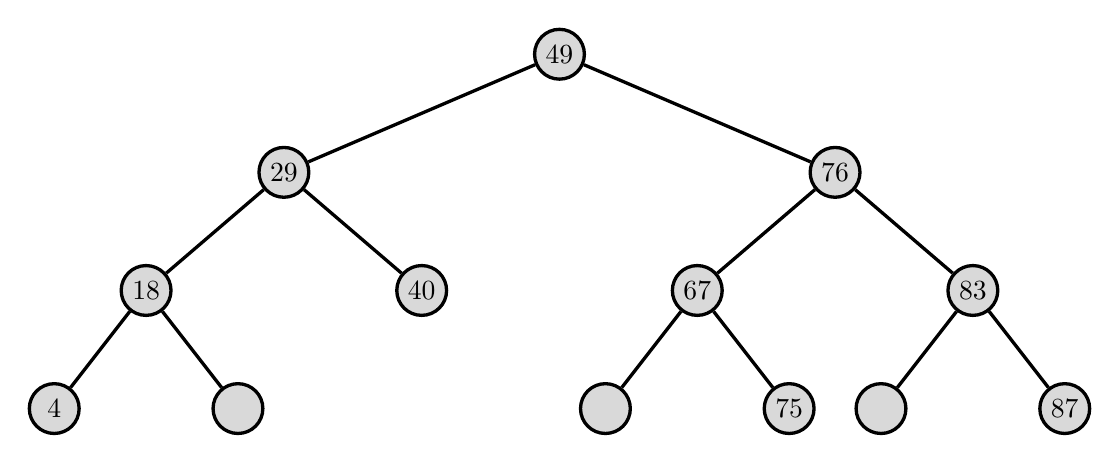
\begin{tikzpicture}[very thick,level/.style={sibling distance=70mm/#1}]
% root
\node [vertex] (r){$49$}
	% left subtree
	child {
		node [vertex] (a) {$29$}
		child {
			node [vertex] {$18$}
			child {
				node [vertex] {$4$}
      		}
      		child {
      			node [vertex] {}
      		}
    	}
		child {
			node [vertex] {$40$}
    	}
	}
	% right subtree
	child {
		node [vertex] {$76$}
		child {
			node [vertex] {$67$}
			child {
				node [vertex] {}
			}
			child {
				node [vertex] {$75$}
			}
		}
		child {
			node [vertex] {$83$}
			child {
				node [vertex] {}
			}
			child {
				node [vertex] {$87$}
			}
		}
	};
\end{tikzpicture}
\end{figure}
\begin{figure}[H]
\centering
\caption{\mintinline{bash}{bigTree} binary search tree}
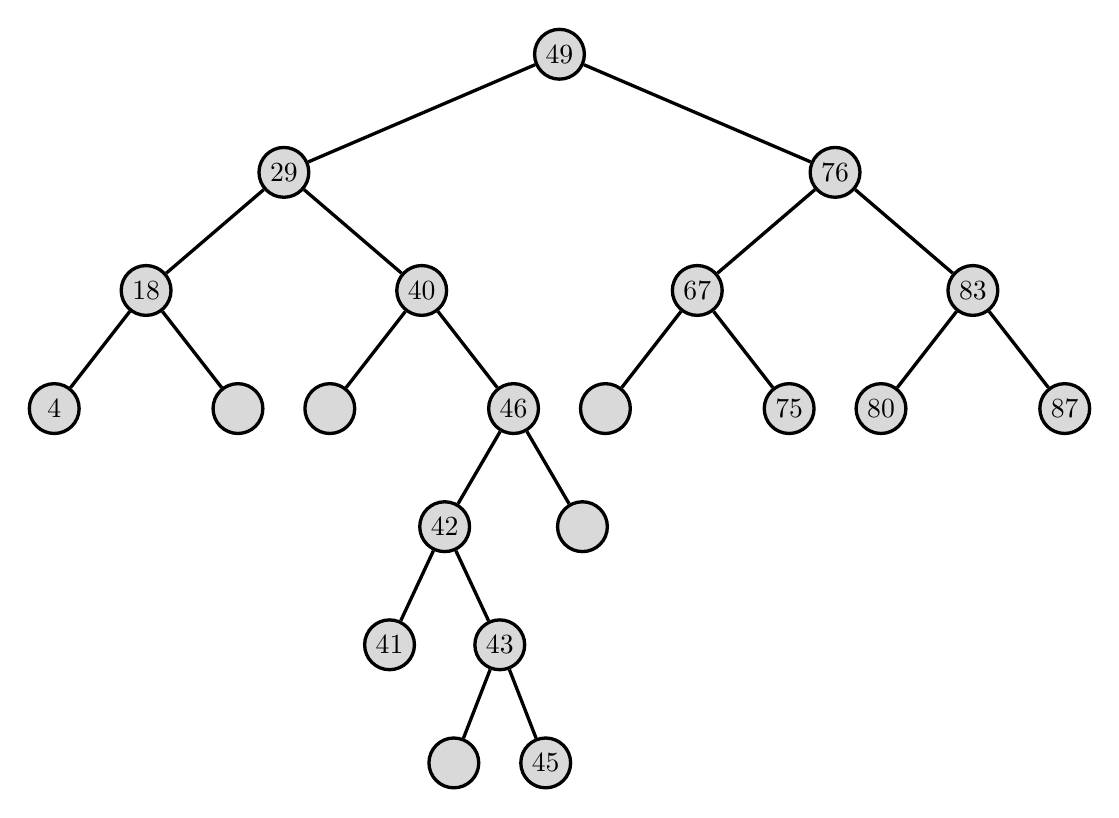
\begin{tikzpicture}[very thick,level/.style={sibling distance=70mm/#1}]
% root
\node [vertex] (r){$49$}
	% left subtree
	child {
		node [vertex] {$29$}
		child {
			node [vertex] {$18$}
			child {
				node [vertex] {$4$}
			}
			child {
				node [vertex] {}
			}
		}
		child {
			node [vertex] {$40$}
			child {
				node [vertex] {}
			}
			child {
				node [vertex] {$46$}
				child {
					node [vertex] {$42$}
					child {
						node [vertex] {$41$}
					}
					child {
						node [vertex] {$43$}
						child {
							node [vertex] {}
						}
						child {
							node [vertex] {$45$}
						}
					}
				}
				child {
					node [vertex] {}
				}
			}
		}
	}
	% right subtree
	child {
		node [vertex] {$76$}
		child {
			node [vertex] {$67$}
			child {
				node [vertex] {}
			}
			child {
				node [vertex] {$75$}
			}
		}
		child {
			node [vertex] {$83$}
			child {
				node [vertex] {$80$}
			}
			child {
				node [vertex] {$87$}
			}
		}
	};
\end{tikzpicture}
\end{figure}

\newpage
\subsection{Binary search tree traversal}

The traversal methods of pre-order, in-order and post-order were supplied as existing code, and therefore only the console output will be shown.

\subsubsection{Traversal console output}

The following console output demonstrates the insertion of values, pre-order, in-order and post-order traversals of \mintinline{bash}{tree}.
\\
\begin{consolecode}
Inserting the following values to tree: 
49 76 67 29 75 18 4 83 87 40 

Pre-order traversal of tree:
49 29 18 4 40 76 67 75 83 87 

In-order traversal of tree:
4 18 29 40 49 67 75 76 83 87 

Post-order traversal of tree:
4 18 40 29 75 67 87 83 76 49 
\end{consolecode}

\noindent
The following console output demonstrates the insertion of values, pre-order, in-order and post-order traversals of \mintinline{bash}{bigTree}.
\\
\begin{consolecode}
Inserting the following values to bigTree: 
49 76 67 29 75 18 4 83 87 40 80 46 42 43 45 41 

Pre-order traversal of bigTree:
49 29 18 4 40 46 42 41 43 45 76 67 75 83 80 87 

In-order traversal of bigTree:
4 18 29 40 41 42 43 45 46 49 67 75 76 80 83 87 

Post-order traversal of bigTree:
4 18 41 45 43 42 46 40 29 75 67 80 87 83 76 49
\end{consolecode}

\newpage
\subsection{Print leaf nodes only}

A leaf node of a binary tree is a node which does not reference a left node, and does not reference a right node. The following \emph{recursive} method has been created to print all the leaf nodes in a binary search tree. The method utilizes in-order traversal.

\subsubsection{Print leaf nodes only Java method}

\begin{listing}[H]
\caption{Print leaf nodes only method}
\begin{javacode}
// public method, initiates recursive printLeafHelper()
public synchronized void printLeafOnly() {
    printLeafHelper(root);
}

// private recursive method which traverses the tree
private synchronized void printLeafHelper(TreeNode node) {
    if(node == null) {
        return;
    }

    printLeafHelper(node.left);

    // only print data if left and right are null
    if(node.left == null && node.right == null) {
        System.out.print(node.data + " ");
    }

    printLeafHelper(node.right);
}
\end{javacode}
\end{listing}

\subsubsection{Print leaf nodes only console output}

The following console output demonstrates the execution of Java code 4.1 with the original \mintinline{bash}{tree} binary search tree.
\\
\begin{consolecode}
Print leaf nodes only for tree:
4 40 75 87 
\end{consolecode}

\noindent
The following console output demonstrates the execution of Java code 4.1 with the \mintinline{bash}{bigTree} binary search tree.
\\
\begin{consolecode}
Print leaf nodes only for bigTree:
4 41 45 75 80 87 
\end{consolecode}

\newpage
\subsection{Print non-leaf nodes only}

A non-leaf node is the inverse of a leaf node in a binary tree. A non-leaf node references either a left, or right node. The following \emph{recursive} method has been created to print all non-leaf nodes within a binary search tree. The method utilizes in-order traversal.

\subsubsection{Print non-leaf nodes only Java method}

\begin{listing}[H]
\caption{Print non-leaf nodes only method}
\begin{javacode}
// public method, initiates recursive printNonLeafHelper()
public synchronized void printNonLeafOnly() {
    printNonLeafHelper(root);
}

// private recursive method which traverses the tree
private synchronized void printNonLeafHelper(TreeNode node) {
    if(node == null) {
        return;
    }

    printNonLeafHelper(node.left);

    // only print data if left or right != null
    if(node.left != null || node.right != null) {
        System.out.print(node.data + " ");
    }

    printNonLeafHelper(node.right);
}
\end{javacode}
\end{listing}

\subsubsection{Print non-leaf nodes only console output}

The following console output demonstrates the execution of Java code 4.2 with the original \mintinline{bash}{tree} binary search tree.
\\
\begin{consolecode}
Print non-leaf nodes only for tree:
18 29 49 67 76 83 
\end{consolecode}

\noindent
The following console output demonstrates the execution of Java code 4.2 with the \mintinline{bash}{bigTree} binary search tree.
\\
\begin{consolecode}
Print non-leaf nodes only for bigTree:
18 29 40 42 43 46 49 67 76 83 
\end{consolecode}

\newpage
\subsection{Print height of tree}

The height (also known as depth) of a binary search tree is the depth of the deepest node in a binary search tree. The following \emph{recursive} method is an adaptation of a Java method by \citet{Flaschen2014}. The method has been modified to follow convention that if a binary tree is empty, the method will return $-1$ \citep[p. 239]{Watt2001}.

\subsubsection{Print height of tree Java method}

\begin{listing}[H]
\caption{Print height of tree method}
\begin{javacode}
// public method, initiates recursive getHeightHelper()
public synchronized int getHeight() {
    return getHeightHelper(root);
}

// adaptation of Flaschen's method (2014)
private synchronized int getHeightHelper(TreeNode node) {
    if(node == null) {
        return -1;
    }

    if(node.left == null && node.right == null) {
        return 0;
    }

    return Math.max(getHeightHelper(node.left), getHeightHelper(node.right)) + 1;
}
\end{javacode}
\end{listing}

\subsubsection{Print height of tree console output}

The following console output demonstrates the execution of Java code 4.3 with the \mintinline{bash}{tree} binary search tree.
\\
\begin{consolecode}
Print height of tree:
3
\end{consolecode}

\noindent
The following console output demonstrates the execution of Java code 4.3 with the \mintinline{bash}{bigTree} binary search tree.
\\
\begin{consolecode}
Print height of bigTree:
6
\end{consolecode}

\noindent
The following console output demonstrates the execution of Java code 4.3 where a binary search tree is either empty, or only contains the root node.
\\
\begin{consolecode}
Print height of emptyTree:
-1

Print height of oneNodeTree:
0
\end{consolecode}
%\section{Conclusion}

This literature review has explored the differences between genders in the use of SNS, and has identified key differences in user motivation. Studies have shown that men are more likely to perform information-based activities on SNS than women, which align with the social gender role framework introduced by \citet{Eagly1987}. Men are also more open to expanding their networks and use SNS as a tool to create new relationships, and more frequently use SNS as a dating platform than women. Women on the other hand, have been found to use SNS to maintain current relationships, and are generally more predisposed than men to provide emotional support to their friends. Women are attracted to the socialising aspect of SNS, and recent studies have shown that women have a larger social network than men. These key differences are also consistent with social gender theory.

All but one study within the scope of this review used self-reported data from their respondents. \citetapos{Haferkamp2012} research included observed data, and although the results were consistent with findings from other studies, there is insufficient literature within this review to conclude that self-reported data and observed data will yield similar results. There are opportunities to conduct further research based on observed data, however questions regarding user privacy would have to be raised, with the amount of personal information available on SNS.

CMC competency as a variable was not found in any of the studies relating to gender in this review. \citet{Ross2009} measured CMC competency, however the research focused on the effect of personality on SNS users and did not exhibit any correlations between gender.

\citet[p. 897]{Kimbrough2013} succinctly pointed out that while users have the ability to choose to behave in any way they wish online, men and women still conform to behaviour that is consistent with ``social role expectations'' from the offline world. This literature review has identified some motivational differences in the use of SNS and compared them to social gender role expectations with the aim of better understanding the differences between genders in SNS use.

\newpage
\urlstyle{rm}
\bibliographystyle{apacite}
\addcontentsline{toc}{section}{References}
\bibliography{./bib/Year_1-Sem_2-CSP2348-A2}


\end{document}